\chapter{Extraction de Données Relatives aux Demandes}
\label{chap:quanta}

\section{Introduction}
\label{sec:quanta:introduction}
Au c\oe{}ur de l'analyse des décisions de justice se trouve le concept de demande. Il s'agit d'une réclamation ou requête effectuée par une des parties devant le juge. Par exemple, une partie peut demander des dommages-intérêts en réparation d'un préjudice subi, ou bien un divorce, ou bien des indemnités auxquelles elle pense avoir droit, ou encore une étude d'expert ... Les demandes sont fondamentales car l'argumentation durant le déroulement de l'affaire a deux buts : faire accepter ses demandes et faire rejeter celle de la partie adverse. L'extraction des demandes et des résultats correspondant, dans un corpus, permet ainsi d'avoir une estimation quantifiée de la décision des juges sur des types de demandes. Les informations qui nous intéressent sont la \textbf{catégorie de la demande}, le \textbf{quantum ou montant demandé}, le \textbf{sens du résultat} (la demande a-t-elle été acceptée ou rejetée?), et le \textbf{quantum ou montant obtenu} (décidé par les juges). Pour pouvoir extraire les demandes et les résultats, il est nécessaire de comprendre comment ils sont exprimés et co-référencés dans les décisions jurisprudentielles. Leur expression peut comporter plus ou moins de complexité avec souvent des références à des jugements antérieurs, des agrégations ou des restrictions (Figure \ref{fig:quanta:expr-dmd-rst}).

\subsection{Données cibles à extraire}
\subsubsection{Catégorie de demande}
Une catégorie $c$ de demande regroupe les prétentions qui sont de même nature par le fait qu'elles partagent deux aspects: l'\textbf{objet} demandé (par ex. dommages-intérêts, amende, déclaration de créance, ...) et le \textbf{fondement} c'est-à-dire les règles ou normes ou principes juridiques qui fondent la demande (par ex. article 700 du code de procédure civile). Des expressions particulières sont souvent utilisées pour faire référence aux catégories (Tableau \ref{tab:quanta:exemple-categorie}).

\begin{table}[h!]
\scriptsize
\begin{tabular}{|p{0.45\textwidth}|p{0.15\textwidth}|p{0.3\textwidth}|}
\hline
\textbf{Expression nominative (label)  }                                     & \textbf{Objet}                                                       & \textbf{Fondement}                                                                 \\ \hline
dommages-intérêts pour abus de procédure (danais)                    & dommages-intérêts                                           & Articles 32-1 code de procédure civile + 1382 code de procédure civile \\ \hline
amende civile pour abus de procédure (acpa)                        & amende civile                                               & Articles 32-1 code de procédure civile + 559 code de procédure civile  \\ \hline
frais irrépétibles  (styx)                                        & dommages-intérêts                                           & Article 700 du code de procédure civile                                 \\ \hline
dommages-intérêts pour trouble de voisinage (doris)                 & dommages-intérêts                                           & principe de responsabilité pour trouble anormal de voisinage           \\ \hline
déclaration de créance au passif de la procédure collective (dcppc) & déclaration de créance & L622-24 code de commerce                                               \\ \hline
dommages-intérêts pour concurrence déloyale (concdel)                  & dommages-intérêts                                           & Article 1382 du code civil                                             \\ \hline
\end{tabular}
\caption{Exemples de catégories de demandes}\label{tab:quanta:exemple-categorie}
\end{table}

\subsubsection{Quantum demandé}
Le quantum demandé quantifie l'objet de la demande. Nous le notons $q_d$. Par exemple, dans l'exemple de la Figure \ref{fig:quanta:expr-dmd}, "3000 \euro{}" est le quantum demandé pour dommages-intérêts pour procédure abusive. Bien que, dans cette étude, nous ne nous intéressons particulièrement qu'aux montants d'argent, le quantum peut être une durée (garde d'enfant, ou emprisonnement, ...). Toutes les catégories demandes n'ont pas un quantum (par ex. une demande de divorce) et seul le sens du résultat sera la données à extraire dans ce cas.

\subsubsection{Sens du résultat}
Le sens du résultat est l'interprétation de la réponse des juges à une demande. Nous le notons $s_r$. En général, le sens peut être positif si la demande a été \textbf{acceptée} ou négatif si la demande a été \textbf{rejetée}. Il arrive aussi que le résultat soit reporté à un jugement futur (un \textbf{sursis à statuer} est alors prononcé). 

\subsubsection{Quantum obtenu ou quantum résultat}
Le quantum obtenu quantifie le résultat ou la réponse des juges. Nous le notons $q_r$. Il est en général inférieur ou égal au quantum demandé. Si la demande est rejetée, le quantum est évidemment nul. il doit être de la même nature que le quantum demandé (montant d'argent ou durée).

\subsection{Expression, défis et indicateurs d'extraction}
Les demandes sont décrites à la fin de la section d'exposé des faits, procédures, moyens et prétentions des parties (section LITIGE). Elles rentrent donc dans les "moyens et prétentions des parties" qui regroupent les demandes et les arguments des parties. Quant aux résultats, ils sont décrits dans la section DISPOSITIF et dans la section MOTIFS (raisonnement des juges). Les demandes sont exprimées en paragraphe où chaque paragraphe correspond soit à une partie, soit à un groupe de partie partageant les mêmes demandes (par ex. des époux). Le paragraphe est parfois organisé en liste dont chaque élément exprime une ou plusieurs demandes, ou fait référence à un jugement antérieur. Les résultats ont aussi la forme de liste dans la section DISPOSITIF. Par contre, dans les motifs de la décision, les raisonnements sont organisés en paragraphes, et ordonnés catégorie après catégorie. Le résultat est donné à la fin du groupe de paragraphes associé à la catégorie.

\begin{figure}[h]
\scriptsize
\centering
\begin{subfigure}[t]{0.95\textwidth}
\fbox{\parbox{\textwidth}{Jennifer M., Catherine M. et Sandra M. ... demandent à la Cour de :

- les recevoir régulièrement appelantes incidentes du \textcolor{blue}{jugement du 23/05/2014} ;

- infirmer \textcolor{blue}{le dit jugement} en \textcolor{brown}{toutes ses dispositions} ; ...

Statuant à nouveau ...

- \textcolor{brown}{les condamner au paiement d'une somme de  3 000,00 \euro{} pour procédure abusive et aux entiers dépens} ; }}
\caption{Exemples d'expression de demandes}\label{fig:quanta:expr-dmd}
\end{subfigure} 


\begin{subfigure}[t]{0.95\textwidth}
\fbox{\parbox{\textwidth}{La cour, ...  

CONFIRME \textcolor{blue}{le jugement entreprise} en \textcolor{brown}{toutes ses dispositions}.

Y ajoutant

\textcolor{gray}{CONSTATE que Amélanie Gitane P. épouse M. est défaillante à rapporter la preuve
d'une occupation trentenaire lui permettant d'invoquer la prescription
acquisitive de la parcelle BH 377 située [...].}

\textcolor{gray}{DEBOUTE Amélanie Gitane P. épouse M. de sa demande en dommages et intérêts.}

\textcolor{gray}{CONDAMNE Amélanie Gitane P. épouse M. aux dépens d'appel.}

\textcolor{gray}{DIT n'y avoir lieu à l'application de l'article 700 du Code de Procédure Civile.}
}}
\caption{Exemple d'expression de résultat}\label{fig:quanta:expr-rst}
\end{subfigure}
\caption{Expressions \textcolor{gray}{simples}, ou comprenant des  \textcolor{blue}{références} et  des \textcolor{brown}{agrégations} (extraits de la décision 14/01082 de la cour d'appel de Saint-Denis (Réunion))}\label{fig:quanta:expr-dmd-rst}
\end{figure}
 Cette pseudo-structure n'est pas standard et elle impose de nombreux défis à relever. D'une part, la séparation des demandes et des résultats rend difficile la résolution de référence entre prétentions et résultats. En effet, une décision jurisprudentielle porte sur plusieurs demandes de catégorie différentes dont il faut identifier la catégorie, le quantum demandé, le sens du résultat et le quantum obtenu. Il est important de faire correspondre un quantum demandé extrait au sens et au quantum du résultat qui font référence à la même demande. Le problème de co-référence est généré aussi par la redondance; par ex. les résultats exprimés dans les MOTIFS sont résumés dans le DISPOSITIF. D'autre part, les références aux jugements antérieurs exigent de résoudre des références aux résultats de jugements antérieurs qui sont, heureusement, rappelés dans le même document. Notons aussi que les difficultés liés aux agrégations (par ex. "\textit{infirmer ... en toutes ces dispositions}") et aux restrictions/sélections (par ex. "\textit{infirme le jugement ... sauf en ce qu'il a condamné M. A. ...}") devraient être résolues. Par ailleurs, les catégories de demandes sont nombreuses (500+ code NAC(?)) mais ne sont pas toutes présentes dans toutes les décisions. Toutes ses contraintes démontrent bien la diversité et l'état non-structuré des documents. Elles induisent des difficultés pour l'annotation manuelle de suffisamment données de référence et la modélisation de l'approche d'extraction. Cependant, nous avons remarqué quelques indicateurs qui pourraient être exploité implicitement ou explicitement.

Nous nous sommes intéressés aux demandes dont les quanta sont des sommes d'argent. Les mentions de somme d'argent suivent généralement la forme "\verb=NOMBRE MONNAIE=" (par ex. 3000 \euro{}, 15 503 676 francs, un euro, 339.000 XPF). Nous remarquons que les nombres sont très rarement écrites en lettre. Ainsi, en répertoriant les unités monétaires mentionnées dans les décisions, il est possible d'annoter les sommes d'argent à l'aide d'une expression régulière (Équation \ref{equation:quanta:regex-argent}) (?)\textcolor{red}{évaluation}.
\begin{equation} %\scriptsize
\splitdfrac{\backslash [0-9](\backslash [0-9]|[',.]|\backslash s)*}{(euro[s]\left\{0,1\right\}|franc[s]\left\{0,1\right\}|\euro{}|F|CFP|XPF|EUR|EUROS)( |\$)}\label{equation:quanta:regex-argent} % Ђ 
\end{equation}
%\texttt{\small $\backslash$p{Digit}($\backslash$p{Digit}|[',.]|\ $\backslash$s)*(euro[s]{0,1}|franc[s]{0,1}|\euro{}|F|CFP|EUR|EUROS)( |\$)}
La terminologie utilisée est aussi un bon indicateur des demandes et résultats. En effet, le vocabulaire utilisé est très souvent propre aux types de demandes, et réciproquement, ce vocabulaire permet d'exprimer des demandes de même nature. Par exemple le dernier élément de la Fig. \ref{fig:quanta:expr-dmd} comprend le terme "\textit{pour procédure abusive}" qui est près d'une somme d'argent (\textit{3000 \euro{}}); il est donc probable que ce type de terme assez particulier soit un bon indicateur de la position des quanta. Par ailleurs, des verbes particuliers sont utilisés pour exprimer les prétentions et résultats : infirmer, confirmer, constater, débouter, dire, ... Comme autres formes récurrentes, on pourrait citer l'ordre des demandes (resp. résultats). Généralement, on a les constats, les références aux jugements antérieurs, les demandes principales (?) et secondaires (?).

\section{Formulation du problème}
\label{sec:quanta:formulation}
Pour formuler le problème, nous avons tenu compte principalement de deux aspects:
\begin{enumerate}
    \item la présence de plusieurs demandes de catégories similaires et différentes dans une même décision;
    \item l'existence d'un grand nombre de catégories (500+); ce qui rend difficile l'annotation d'un jeu de données de référence pour couvrir toutes ces catégories.
\end{enumerate}

Nous avons par conséquent opter pour la définition d'approches génériques adaptables à chaque catégorie. L'idée est de pouvoir  traiter progressivement les catégories et par conséquent, annoter progressivement des données de référence. Chaque exécution des approches définies permet ainsi d'extraire uniquement les demandes d'une seule catégorie. L'annotation manuelle d'exemples a été par conséquent définie par catégorie afin que la tâche soit plus facile pour les experts. Le protocole d'annotation se déroule en étapes: 
\begin{enumerate}
    \item choix d'une catégorie: définition d'un nom, de l'objet et du fondement;
    \item recherche par mots-clés des documents susceptibles de contenir la catégorie (par exemple sur le site internet de LexisNexis);
    \item parmi les documents trouvés, choisir quelques uns de ceux qui contiennent effectivement des demandes de la catégorie; 
    \item lire chaque document choisi pour identifier toutes les demandes présentes de la catégories tout en remplissant le tableau des demandes de références dont un extrait est illustré par le Tableau \ref{tab:quanta:tab-annotations}.
\end{enumerate}

\begin{table}[!htb]
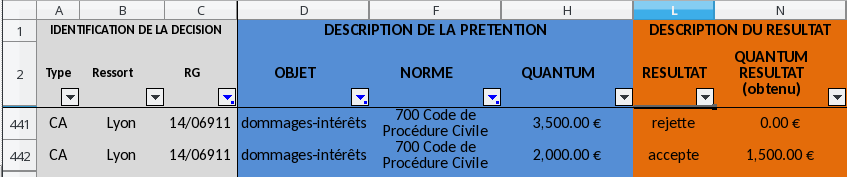
\includegraphics[width=\textwidth]{tab-annotations.png}
\scriptsize{Les noms des champs sont sur les 2 premières lignes et les demandes sont données en exemple pour la catégorie \textit{dommages-intérêts sur le fondement de l'article 700 du code de procédure civile} (décision 14/06911 de la cour d'appel de Lyon).}
\caption{Structure et extrait du tableau d'annotations manuelles des demandes.} \label{tab:quanta:tab-annotations}
\end{table}

Le problème est ainsi décomposé grossièrement en tâches:
\begin{description}
\item[Tâche 1:] Détection des catégories présentes dans le document pour n'appliquer l'extraction  que de ces catégories;
\item[Tâche 2:] Extraction des demandes des catégories identifiées:
\begin{enumerate}
	\item identification des données: quanta demandés, quantas obtenus, et sens du résultat;
	\item résolution des références ou des liens entre données de la même demande.
\end{enumerate}
\end{description}

L'annotation des sommes d'argent doit être réalisée préalablement à la 2$^\text{ème}$ tâche.

 Dans la section suivante, nous synthétisons l'analogie avec des problématiques couramment traités et explorons les approches proposées dans des travaux publiés.

\section{Travaux connexes}
\label{sec:quanta:biblio}
Chacune de ses tâches se rapproche d'une tâche traitée dans la littérature, et nous donne ainsi des voies de solution. En effet, la détection de catégories dans les décisions peut être modélisée comme un problème de classification de document. Les deux dernières tâches se rapprochent plus de problématiques d'extraction d'entités complexes à champs/attributs comme l'extraction d'évènements, le remplissage de champs, ou encore l'extraction d'entités ou de rôles sémantiques et la résolution de référencement.

\subsection{Problèmes analogues: inférence de structures}% avec des problématiques d'extraction d'information}

Les demandes ressemblent aux structures complexes de la littérature sur l'extraction d'information. Le concept qui semble le plus similaire est celui d'évènement. Il s'agit probablement de l'une des structures les plus complexes de l'extraction d'information. Plusieurs campagnes en ont fait l'objet de compétitions par des définitions et des catégorisations et caractérisations aussi précises que possibles. La campagne \citep{ace2005event}, par exemple, structure un évènement en lui associant un type, un énoncé, des déclencheurs, des arguments, et des attributs. Nous retrouvons des composants respectivement similaires chez les demandes (Tableau \ref{tab:quanta:analogieevt}): la catégorie, les passages d'énoncés de demande et résultat, les termes-clés caractéristiques de la catégorie (sa famille de termes en quelque sorte), les quanta comme arguments et le sens du résultat comme attribut (plus précisément comme polarité).


Mais ces formulations ne couvrent pas toujours avec exhaustivité l'expressivité des énoncés d'évènements. En effet, certains travaux se limitent à une extraction généralement limitée au niveau d'une phrase et très peux s'essayent à proposer des solutions à l'échelle d'un document ou d'un corpus pour les situations où les données ne se trouvent pas toutes dans une même phrases. Ainsi, plus la portée est grande plus la tâche est complexe. C'est pourtant bien cette complexité qui caractérise les données réelles. 
\begin{itemize}
\item Extraction d'évènement : 
\end{itemize}
\begin{table}[h]
\small
\begin{tabular}{|p{0.2\textwidth}|p{0.3\textwidth}|p{0.4\textwidth}|}
\hline
\textbf{Champs} & \textbf{\cite{ace2005event}} & \textbf{Analogie chez les demandes} \\ \hline
\textbf{Type} &  Die & Catégorie="Dommages-intérêts pour procédure abusive" \\ \hline
\textbf{Passage} (\textit{extend}) & "Il est mort hier d'une insuffisance rénale."  & (\textit{Figure \ref{fig:quanta:expr-dmd-rst}}) \\ \hline
\textbf{Déclencheur} & "mort" & "procédure abusive"\\ \hline
\textbf{Argument} & Victim-Arg="il" \linebreak Time-Arg="hier"  & Quantum-demandé="3000\euro{}"\linebreak  Quantum-obtenu="0 \euro{}"\ \\ \hline
\textbf{Attribut} & Polarity=POSITIVE, Tense=PAST & Sens-résultat="Rejeté" \\ \hline
\end{tabular}
\caption{Exemple d'analogie entre les évènements et l'extraction de demande} \label{tab:quanta:analogieevt}
\end{table}
\begin{itemize}
\item Remplissage de champs des entités \textbf{Demande} (\textit{slot-filling)}: \textbf{Catégorie, Quantum-demandé, Quantum-obtenu, Sens-résultat}
\item Extraction d'entités et relations ou résolution de référence: par ex. \textbf{(quantum demandé, quantum obtenu)}
\end{itemize}

\subsection{Approches d'extraction de structures}
L'extraction d'information composée passe par une formulation modulaire du problème en tâches plus simples. Par exemple, on a d'abord l'extraction respective déclencheurs, les arguments et les attributs. Ensuite, la résolution de référence vient construire les structures en reliant les différents valeurs de champs extraites précédemment. A partir de là, on définit une approche d'extraction qui peut modéliser soit une chaine de d'inférences élémentaires ou pipeline, soit une inférence jointe capable d'extraire toute la structure d'un seul coup. Les pipelines sont une approximation grossière victime de la propagation d'erreurs entre module [?]. Bien que les modules sont simples, ils ne corrigent malheureusement pas les erreurs des niveaux précédents. L'inférence jointe permet non seulement d'éviter ou de réduire tout au moins la propagation d'erreurs mais aussi d'exploiter la dépendance mutuelle qui existe entre les étages [?]. Cependant, ce n'est pas toujours une bonne idée de joindre tous les modules; il faut bien choisir les étapes à joindre.


\begin{table}[!h]
\small
\begin{tabular}{|p{0.25\textwidth}|p{0.7\textwidth}|}
\hline
\textbf{Type d'approches} & \textbf{Exemples} \\ \hline
\textbf{Chaine de traitement} & \textbf{Chaîne de classifieurs  }\cite{ahn2006stages} \\ \hline
\textbf{Modélisation probabiliste} de la structure de l'évènement & \textbf{Modèle joint d'inférence} des entités, arguments, déclencheurs

$p_\theta(t_i, r_i, a \vert i, N_i, x)$ \cite{yang2016jointEntityEvt} %\linebreak 
\\ \hline
\textbf{Réseau de neuronnes} pour automatiser la génération des caractéristiques et la modélisation de la structure & (i) \textbf{Architecture multicouche de réseaux de neuronnes récurrents}: encodage de la phrase, encodage des contextes, prédiction du déclencheur, prédiction des rôles, mémoire matricielle d'interdépendance déclencheur-argument \cite{nguyen2016jointtrgarg},  

(ii) \textbf{Réseau de pointeur} (\textit{pointer network}): un encodeur de la phrase et des contextes, plusieurs décodeurs (un pour chaque champ) \cite{palm2017e2e-dnn} \\ \hline
\end{tabular}
\caption{Type d'approches}
\end{table}


\subsection{Extraction de la terminologie d'un domaine}
La recherche sur l'extraction des évènements s'appuie sur l'identification des termes-clés, appelés déclencheurs, caractéristiques des types d'évènements car ils semblent être des indicateurs incontournables non seulement de l'énoncé mais aussi les repères de localisation des arguments. Qu'ils soient identifiés au préalablement ou conjointement avec les arguments, les déclencheurs sont jusqu'à présent appris de manière supervisée c'est-à-dire à partir d'exemples annotés manuellement de déclencheurs dans des exemples d'énoncés d'évènement. L'annotation manuelle de tels termes étant fastidieuse et risquant de manquer d'exhaustivité dans les cas de données réelles, il serait préférable de les apprendre lorsqu'on ne dispose pas d'exemples de déclencheurs. C'est notamment notre situation, où nous avons besoin des termes caractéristiques des catégories de demandes. Fort heureusement, la recherche d'information, l'apprentissage d'ontologie et d'autres tâche d'analyse de texte comme la classification de documents ont encourager le développement d'approches d'extraction de termes-clés. On distingue principalement les filtres d'une part et les méthodes statistiques d'autres part.


\subsubsection{Filtres}
% LISTES TERMES EXTRAITS POUR CHAQUE CATÉGORIE
\subsubsection{Méthodes statistiques}
% LISTES POUR CHAQUE CATÉGORIE
\begin{table} 
	\caption{Métriques globales de termes: les métriques supervisées sont notées $f(t_k,c_i)$ et les non-supervisées sont notées $g(t_k)$} \label{tab:quanta:globalweights}
	\scriptsize
	\begin{tabular}{p{0.48\textwidth}@{\hskip 0.2in}p{0.45\textwidth}}
		\hline\noalign{\smallskip}
		Description & Formule \\
		\noalign{\smallskip}
		\hline
		\noalign{\smallskip}
		Inverse document frequency \cite{sparck1972idf}: simply computes the importance score of $t_k$ all over a corpus $D$ & $idf(t_k) = \log_2 (\frac{N}{N_{t_k}})$  \\ \noalign{\smallskip}
		Delta Document Frequency & $deltadf(w,c_i) = DF_{t_k,c_i} - DF_{t_k,\overline{c_i}}$\\ \noalign{\smallskip}
		Test of Marascuilo & $mar(t_k, c_i) = $ \begin{equation*} 
		\,
		\dfrac{\left(
			\splitdfrac{\splitdfrac{\splitdfrac{(N_{t_k,c_i} - N_{t_k}N_{t_k,c_i}/N)^2}{+ (N_{t_k,\overline{c_i}} - N_{t_k}N_{\overline{c_i}}/N)^2}}{+ (N_{\overline{t_k},c_i} - N_{c_i}N_{\overline{t_k}}/N)^2}}{+ (N_{\overline{t_k},\overline{}} - N_{\overline{t_k}}N_{\overline{c_i}}/N)^2}\right)}{N}
		\end{equation*} \\ \noalign{\smallskip}
		Chi square & $chi2(t_k,c_i) = \frac{N ((N_{t_k,c_i} N_{\overline{t_k},\overline{c_i}}) - (N_{t_k,\overline{c_i}} N_{\overline{t_k},c_i}))^2}{N_{t_k} N_{\overline{t_k}} N_{c_i} N_{\overline{c_i}}}$ \\ \noalign{\smallskip}
		Correlation coefficient of "Ng, Goh, Low" \cite{ng1997ngl} :   & $ngl(t_k,c_i) = \frac{\sqrt{N} ((N_{t_k,c_i} N_{\overline{t_k},\overline{c_i}}) - (N_{t_k,\overline{c_i}} N_{\overline{t_k},c_i}))}{\sqrt{N_{t_k} N_{\overline{t_k}} N_{c_i} N_{\overline{c_i}}}}$\\ \noalign{\smallskip}
		Coefficient of "Galavotti, Sebastiani, and Simi"  \cite{galavotti2000gss}& $gss(t_k,c_i) = (N_{t_k,c_i} N_{\overline{t_k},\overline{c_i}}) -  (N_{t_k,\overline{c_i}} N_{\overline{t_k},c_i})$ \\ \noalign{\smallskip}
		Relevance frequency & $rf(t_k, c_i) = \log\left(2 + \frac{N_{t_k, c_i}}{max(1, N_{t_k, \overline{c_i}})}\right)$\\ \noalign{\smallskip}
		Information gain & $ig(t_k, c_i) = $ \begin{equation*}
		\splitdfrac{\splitdfrac{\splitdfrac{(N_{t_k,c_i} * \log (N_{t_k,c_i} / (N_{t_k}N_{c_i})))}
				{+ (N_{\overline{t_k},c_i} * \log (N_{\overline{t_k},c_i} / (N_{\overline{t_k}}N_{c_i})))}}
			{+ (N_{t_k,\overline{c_i}} * \log (N_{t_k,\overline{c_i}} / (N_{t_k}N_{\overline{c_i}})))}}
		{+ (N_{\overline{t_k},\overline{c_i}} * \log (N_{\overline{t_k},\overline{c_i}} / (N_{\overline{t_k}}N_{\overline{c_i}})))}
		\end{equation*} \\ \noalign{\smallskip}
		Kulback-Leibler divergence & $kld(t_k, c_i)=(N_{t_k,c_i} / N_{t_k}) * \log (\frac{N_{t_k,c_i} N}{N_{t_k}N_{c_i}})$\\ \noalign{\smallskip}
		Delta Smoothed IDF & $dsidf(t_k, c_i)=\log (\frac{(N_{\overline{c_i}}N_{t_k,c_i}) + 0.5}{(N_{c_i}N_{t_k,\overline{c_i}}) + 0.5} $\\ \noalign{\smallskip}
		Delta BM25 IDF \cite{jones2000bm25idf} & $dbidf(t_k, c_i) = \log (\frac{(N_{\overline{c_i}} - N_{t_k,\overline{c_i}} + 0.5) * (N_{t_k,c_i} + 0.5)}{(N_{c_i} - N_{t_k,c_i} + 0.5) * N_{t_k,\overline{c_i}} + 0.5)} $\\ \noalign{\smallskip}
		\hline
	\end{tabular}
\end{table}
\paragraph{Mesures non-supervisées}
NValue, CValue, IDF et co.
\paragraph{Mesures supervisées}
RF, MARASCUILO, TEST DE PROPORTIONS, CHI2, ...
\subsubsection{Discussions}
\textcolor{red}{PRISE EN COMPTE DE LA LONGUEUR VARIÉE ($\log(l) * f(t)$ ou $l^a * w^b$ / DE L'IMBRICATION / DU CONTEXTE DES TERMES;;;; AFFINER LA LISTE: ENCHAINEMENT FILTRES > MÉTRIQUES STATS > FONCTION CONTRASTIVE}
\cite{LossioVentura2014biotex}, \cite{Bonin2010multiwordncvalue}


\section{Détection des catégories par classification}

Étant données l'ensemble $D_{\overline{c_i}}$ des documents ne comprenant aucune demande de la catégorie d'intérêt $c_i$, nous proposons de modéliser la tâche de détection des catégories en une tâche de classification. Pour chaque catégorie, un classifieur binaire de document est entrainé pour déterminer si le document analysé contient ou pas une demande de la catégorie. Pour cela, chaque document $d_j$ est représenté sous une forme vectorielle traditionnelle du type TF-IDF (\textit{term frequency - inverse document frequency}) où chaque dimension représente un mot dont le poids est le produit normalisé d'un poids $gw$ global au corpus du mot et d'un poids $lw$ local au document: $w(t_k, d_j) = lw(t_k, d_j) \times gw(t_k) \times nf(d_j)$, où $nf$ est le facteur de normalisation. 


\section{Extraction des demandes}
\label{sec:quanta:attributs}

L'étude consiste en la proposition et la comparaison empirique d'adaptations des approches d'extraction de structure à savoir: l'usage de règles, le chainage d'extracteur élémentaire, et l'inférence jointe.


\subsection{Méthode 1: extraction par règles et termes-clés}
\label{subsec:quanta:attributs:regles}

%\textcolor{red}{Cité la localisation des unités de mésure / considérer le découpage en phrases à la place du découpage avec les verbes introductifs. Formaliser l'algorithme (si possible donner la complexité et le temps d'extraction moyen par document)}
Pour chacune des catégories détectées, nous proposons ici une chaine d'extraction à base de termes-clés. Il s'agit d'une approche qui tente de reproduire une lecture naïve du document. Elle est ainsi basée sur des sortes de formes d'expression répétitives et inspirées de nos lectures des documents. La technique consiste à marquer les énoncés de demandes et résultats. Dans ces passages, les quanta sont localisés à proximité de termes-clés caractérisant la catégorie. Par exemple, la Figure \ref{fig:quanta:exemple-proximite} présente un extrait de passage exprimant une demande d'\textit{amende civile pour procédure abusive}.

\subsubsection{Annotation des énoncés et termes-clés}

 La Figure \ref{fig:quanta:exemple-proximite-original} présente l'extrait original et la Figure \ref{fig:quanta:exemple-proximite-marquage} présente le résultat de notre marquage automatique que nous proposons. Les passages, les sommes d'argent, et les termes-clefs sont marqués avec les balises XML resp. \verb=<demande>=, \verb=<argent>=, \verb=<terme-clef>=. Dans cet exemple, on remarque bien que le quantum demandé (\textit{1.500 euros}) se trouve très près de terme-clefs associables à la catégorie \textit{acpa} ("\textit{amende civile}" et "\textit{pour procédure abusive}"). 

\begin{figure}[!htb]
	\scriptsize
	\centering
	\begin{subfigure}[t]{0.95\textwidth}
		\fbox{\parbox{\textwidth}{
				" ... 
				
				- débouter M. S. de ... % l' ensemble de ses demandes
				
				\textbf{- le condamner à payer une amende civile de 1.500 euros pour procédure abusive} ...
				
				- le condamner à payer la somme ..."
		}}
		\caption{Extrait original d'énoncé de demande avant marquage}\label{fig:quanta:exemple-proximite-original}
	\end{subfigure} 
	
	
	\begin{subfigure}[t]{0.95\textwidth}
		\fbox{\parbox{\textwidth}{
				" ... 
				
				- débouter M. S. de ... % l' ensemble de ses demandes
				
				- le \textbf{<demande categorie="acpa">}\underline{condamner} à payer une <terme-clef categorie="acpa">\textbf{amende civile}</terme-clef> de <argent> \textbf{1.500 euros} </argent> <terme-clef categorie="acpa"> \textbf{pour procédure abusive}</terme-clef> ...
				
				- le\textbf{</demande>} \underline{condamner} à payer la somme ..."
		}}
		\caption{Énoncé, sommes d'argent, et termes-clés marqués}\label{fig:quanta:exemple-proximite-marquage}
	\end{subfigure}
	%\caption{Exemple de passage de demande: le quantum demandé est une somme d'argent à proximité des terme-clés}
	\caption{Illustration de la proximité des quantas et termes-clés}
	\label{fig:quanta:exemple-proximite}
\end{figure}

Les énoncés de demande se distinguent de ceux des résultats par leur position dans le document (les demandes dans la section LITIGE et les résultats dans les sections MOTIFS et DISPOSITIF) et par les verbes qui les introduisent (très souvent à l'infinitif pour les demandes et au présent pour les résultats). Nous avons ainsi prédéfini, indépendamment de la catégorie traitée, une liste de mots qui sont généralement des verbes (Tableau \ref{tab:quanta:mots-introductifs}) pour délimiter les demandes et résultats dans leur section respectives. La recherche de passages à l'aide listes de termes n'est pas unique à notre étude. \cite{wyner2010extractlegalelts} utilise par exemple des termes de jugement dans des règles JAPE pour annoter les énoncés de résultats (toute phrase contenant un terme de jugement) : \textit{affirm, grant, deny, reverse, overturn, remand, ...}
\begin{table}
\centering
\scriptsize
 \begin{tabular}{|p{0.28\textwidth}|p{0.3\textwidth}|p{0.12\textwidth}|p{0.11\textwidth}|}
 \hline
 \textbf{Demande} & \multicolumn{3}{c|}{\textbf{Résultat} (organisé par polarité)} \\ \hline
  & \textbf{accepte}  &\textbf{sursis à statuer} & \textbf{rejette}  \\ \hline
 \textit{accorder, admettre, admission, allouer, condamnation, condamner, fixer, laisser, prononcer, ramener, surseoir} & \textit{accorde, accordons, admet, admettons, alloue, allouons, condamne, condamnons, déclare, déclarons, fixe, fixons, laisse, laissons, prononce, prononçons} & \textit{réserve, réservons, sursoit, sursoyons} & \textit{déboute, déboutons, rejette, rejetons} \\ \hline
 \end{tabular}
  \caption{Mots introduisant les énoncés de demandes et de résultats}\label{tab:quanta:mots-introductifs}
 \end{table}

Les termes prédéfinis délimitent les passages de demande et résultat indépendamment de toute catégorie, mais nous ne souhaitons analyser que les passages de la catégorie traitée. Il est donc nécessaire d'identifier les termes-clés indiquant l'expression de cette catégorie. 

\subsubsection{Apprentissage des termes-clés d'une catégorie}

 Nous proposons un apprentissage semi-supervisé de ces termes. L'apprentissage est "supervisé" parce qu'on dispose de 2 corpus annotées pour chaque catégorie $c$: les documents à demande de la catégorie ($D_c$) et des documents sans demande de la catégorie ($D_{\overline{c}}$). L'apprentissage est "semi" parce qu'on ne dispose pas d'exemples de termes caractéristiques de la catégorie, mais uniquement de candidat qui sont en fait les termes de $D_c$. Nous avons utilisé des métriques/tests statistiques d'analyse de proportion pour sélectionner les termes qui sont plus importants dans le corpus $D_c$ que dans $D_{\overline{c}}$. Ces métriques sont listées dans le Tableau \ref{tab:quanta:globalweights}.
 
 \begin{enumerate}
 	\item  pondération et tri décroissant des termes du corpus $D_c \cup D_{\overline{c}}$
 	\item  Sélection des N meilleurs termes (par ex. N=100)
 	\item Filtre des termes donnant le meilleur score sur les données de développement
 \end{enumerate}




\subsection{Méthode 2: classification des sommes d'argent}

\begin{figure}[!htb]
 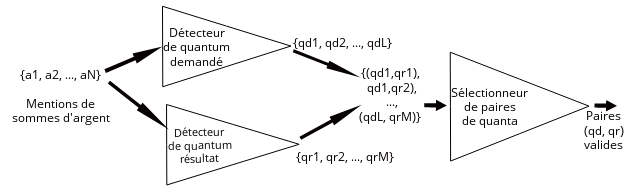
\includegraphics[scale=0.6]{extractDmd-archClassifArgent.png}
 \caption{Extraction des demandes par classification des sommes d'argent}\label{fig:quanta:classif}
\end{figure}

Les deux champs directement accessibles à partir du texte, sont les quanta demandé ($q_d$) et accordé ($q_r$). Pour les demandes à quanta, il est possible de restreindre l'extraction à ces deux variables. Le sens du résultat ($s_r$) est déduit de la valeur extraite du quantum accordé : \[s_r = \left\lbrace \begin{array}{ll}
"accepte" & \text{si } q_r > 0 \\
"rejette" & \text{sinon.} \end{array} \right.\]

L'idée est d'extraire les quanta demandés et obtenus puis de d'identifier les paires $(q_d, q_r)$ qui représentent des demandes. Le système recherche les mentions de sommes d'argent qui sont des quanta. La  détection des quanta est réalisable soit par classification individuelle des sommes d'argent, soit par inférence probabiliste du groupe de quanta. 


La performance d'une telle approche repose sur deux aspects principaux: la définition des  caractéristiques des objets à classifier, et la résolution des doublons. 

\subsubsection{Définition des caractéristiques}

La considération d'une somme d'argent comme quantum dépend de son contexte de mention et de l'histoire globale du document. Nous combinons plusieurs types de caractéristiques:
\begin{itemize}
	\item le plongement sémantique de la somme d'argent;
	\item l'agrégation pondérée du vecteur des mots qui sont dans la phrase de la somme d'argent;
    \item le plongement sémantique de la section
    \item le plongement sémantique du dispositif
    \item le plongement sémantique du document
\end{itemize}

Les caractéristiques des paires consiste en l'agrégation des vecteurs des deux sommes par concaténation, max, ou soustraction.

\subsubsection{Résolution des doublons}
Il s'agit ici des mentions de sommes d'argent à valeurs égales. Certaines sont correspondent au même quantum (par ex. quanta du MOTIFS répétés dans le DISPOSITIF). D'autres représentent des quanta différents.

 Le problème des doublons se pose déjà sur les données d'entrainement. En effet, nous devons retrouver à quelle mention de somme d'argent correspond chaque quantum du tableau des annotations manuelles. Si on annote tous les doublons comme quanta, se retrouve avec des demandes en plus. Même si on considère qu'il s'agit de la même demande, on n'en est pas sûr. On peut choisir le plus probable parmi les doublons présents.

%Résolution des doublons: classification de paires apprise sur un dataset généré à partir du comportement observé des détecteur de quanta sur le corpus d'entrainement. (a1, a2) -> (similaire, différent). UNIQUEMENT POUR DES SOMME DE VALEURS EGALES

\textcolor{red}{STATISTIQUES SUR LE TAUX DE DOUBLONS DANS LES DONNÉES ANNOTÉES}


\subsection{Méthode 3: prédiction jointe de structure}
?Apprentissage sur les documents à une seule demande pour limiter les bruits?

Pré-traitement: normalisation des sommes d'argent dans les document (par ex. 3000 euros <argent valeur="3000 euros">ARGENT\_i</argent> $i$ étant la position d'apparition de la mention)

\begin{equation}
P(D|T,A) = \sum\limits_{i=1}^{\vert D \vert} p_{\theta_1}(d_i = (a_j, a_l) | T, a_j, a_l, A) \cdot p_{\theta_2}(q_{d_i} = a_j | T, a_j, A) \cdot p_{\theta_3}(q_{r_i} = a_l | T, a_l, A)    
\end{equation}

\subsection{Résultats expérimentaux}
\subsubsection{Annotation des données d'évaluation}
\begin{figure}[h!]
	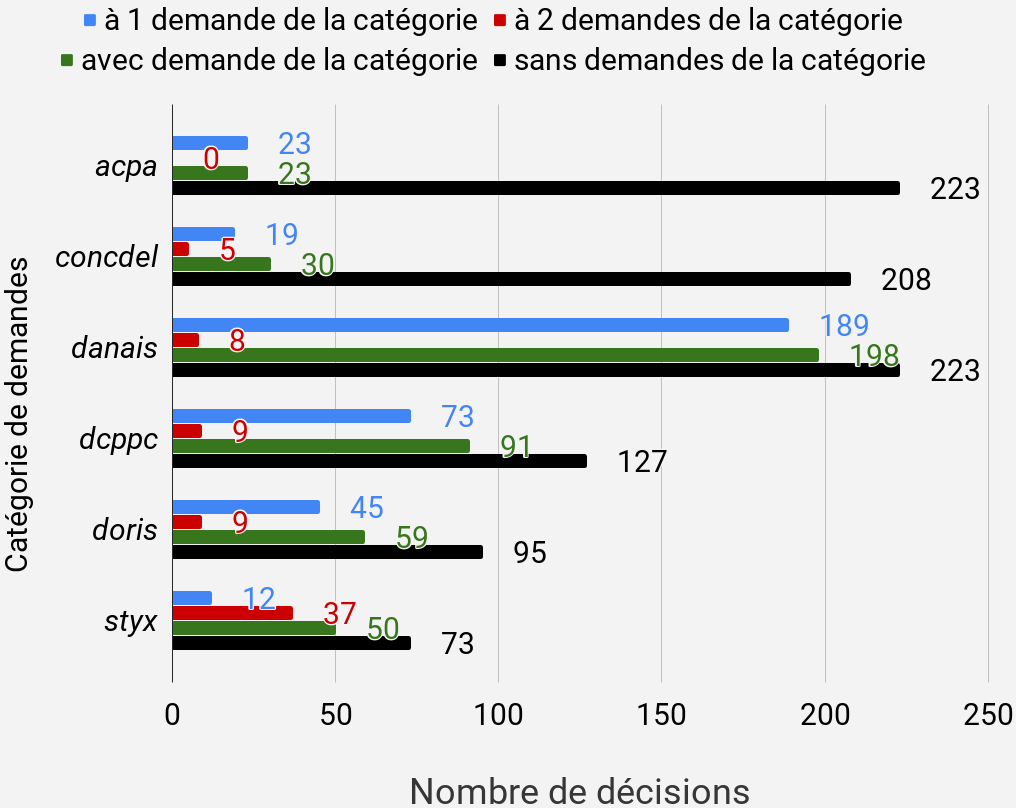
\includegraphics[width=\textwidth]{chartDataset.png}
	\caption{Répartitions des demandes dans les documents annotées pour chaque catégorie.}\label{fig:quanta:hist-repartition-docs}
\end{figure}
Pour une catégorie $c_i$ de l'ensemble $C$ des catégories existantes, les données de références sont annotées dans un tableau. Chaque ligne décrit une demande. L'annotateur devrait associer deux corpus au tableau. Le premier corpus $D_{c_i}$ comprends les documents d'où proviennent les demandes annotées pour $c_i$. Le second corpus $D_{\overline{c_i}}$ contient des exemples de documents ne contenant aucune demande de catégorie $c_i$. Le corpus $D_{\overline{c_i}}$ permet de s'assurer que le système n'extrait pas de demande dans des documents ne discutant pas de $c_i$.  Pour notre étude, un expert a extrait manuellement des demandes des 6 catégories du Tableau \ref{tab:quanta:exemple-categorie}. Nous considérons que les demandes de type $c_i$, présentes dans le corpus $D_{c_i} \cup D_{\overline{c_i}}$, ont été toutes annotées dans le tableau. La répartition, des documents traités durant ce processus, est donnée par l'histogramme de la Figure \ref{fig:quanta:hist-repartition-docs}.  On remarque que, pour toutes les catégories, les documents à une seule demande sont en général majoritaires (barres bleues). Quelques documents ne comprenant aucune demande de la catégorie d'intérêt ont été aussi rassemblés (barres grises). Il faut aussi noter que malgré la non annotation des demandes directement dans les documents mais plutôt dans un tableau (annotation externe), l'annotation reste une tâche très difficile. Le très faible nombre de documents traités en est la conséquence. Le nombre  maximum pour une catégorie n'a été que de 198 documents (barres vertes) \textcolor{red}{[DURÉE D'ANNOTATION? QUELLE EST LA VITESSE MOYENNE D'EXTRACTION MANUELLE DES DEMANDES DANS UN DOCUMENT?]}.



\subsubsection{Métriques d'évaluation}
 Nous évaluons les approches proposées sur l'extraction de 3 données: le quantum demandé $q_d$, le sens du résultat $s_r$ et le quantum obtenu $q_r$. Une demande est donc un triplet $(q_d, s_r, q_r)$. Il est possible d'évaluer le système pour un sous-ensemble $x$ de ce triplet sur les demandes extraites d'un corpus annotées $D$. Nous utilisons les métriques traditionnellement employées en extraction d'information: la précision (Eq. \ref{eq:quanta:precisiondmd}), le rappel (Eq. \ref{eq:quanta:recalldmd}), et la F1-mesure (Eq. \ref{eq:quanta:f1dmd}). 
 \begin{equation}
 Precision_{c_i,x,D} = \frac{TP_{c_i,x,D}}{TP_{c_i,x,D} + FP_{c_i,x,D}}  \label{eq:quanta:precisiondmd}
\end{equation}

\begin{equation}
Rappel_{c_i,x,D} = \frac{TP_{c_i,x,D}}{TP_{c_i,x,D} + FN_{c_i,x,D}} \label{eq:quanta:recalldmd}
\end{equation}

\begin{equation}
F1_{c_i,x,D} =2 \times \frac{Precision_{c_i,x,D} \times Rappel_{c_i,x,D}}{Precision_{c_i,x,D} + Rappel_{c_i,x,D}} \label{eq:quanta:f1dmd}
\end{equation}

Ces mesures sont définies à partir des nombres de vrais positifs ($TP$), faux positifs ($FP$) et faux négatifs ($FN$). Au niveau d'un document $d$:
\begin{itemize}
\item le nombre de vrais positifs $TP_{c_i, x, d}$ est le nombre de demandes extraites de $d$ par le système, qui sont effectivement de la catégorie $c_i$ ;
\item le nombre de faux positifs $FP_{c_i, x, d}$ est le nombre de demandes extraites de $d$ par le système, mais qui ne sont pas des demandes de $c_i$ (demandes en trop);
\item le nombre de faux négatifs $FP_{c_i, x, d}$ est le nombre de demandes annotées comme étant de $c_i$ mais qui n'ont pas pu être extraites par le système (demandes manquées).
\end{itemize}

Au niveau d'un corpus d'évaluation $D$, ces métriques de base sont simplement les sommes de leur correspondant au niveau des documents (Équations \ref{eq:quanta:tpdmd}, \ref{eq:quanta:fpdmd}, et \ref{eq:quanta:fndmd}).

\begin{equation}
TP_{c_i,x,D} = \sum\limits_{d_j \in D} TP_{c_i,x,d_j} \label{eq:quanta:tpdmd}
\end{equation}

\begin{equation}
FP_{c_i,x,D} = \sum\limits_{d_j \in D} FP_{c_i,x,d_j} \label{eq:quanta:fpdmd}
\end{equation}

\begin{equation}
FN_{c_i,x,D} = \sum\limits_{d_j \in D} FN_{c_i,x,d_j} \label{eq:quanta:fndmd}
\end{equation}


La définition de la qualité d'une donnée extraite reste la question fondamentale de l'évaluation. Durant l'annotation, les données sont reportées dans le tableau sous une forme qui peut être différente de la mention dans le document. Par exemple,  La valeur observée et la valeur reportée restent néanmoins égales. Il est donc nécessaire de ne comparer que les valeurs. Pour le sens du résultat, la valeur est catégorique, et par conséquent, facilement comparable. En effet, il suffit de comparer les labels. Par contre, les quanta sont des sommes d'argent i.e. des quantités à valeur et unité monétaire. Pour simplifier, nous avons considéré que l'unité est la même pour les données extraites et annotées pour un même document. Pour obtenir la valeur, nous ramenons la mention extraite à un nombre décimal. Le symbole de la décimale étant la virgule (\og , \fg) en Français, il suffit d'éliminer, de la somme d'argent, tous les caractères différents des chiffres et de la virgule; puis remplacer la virgule par un point. Par exemple, la valeur de \og 3 000 \euro \fg est $3000$, celle de \og 265 ' 550 , 83 euros \fg est $265550.83$ ).



\subsubsection{Détection des catégories par classification}

Nous avons évalué la classification binaire avec quatre classifieurs traditionnels: le classifieur naïf bayésien, l'arbre de décision, les K plus proches voisins (KNN), et la machine à vecteurs de support. A chaque entrainement, s'exécute une sélection de modèle par validation croisée sur les données d'entrainement; elle a pour but de sélectionner la métrique locale et la métrique globale appropriée. Les résultats obtenu par 5-folds cross validation sont présentés sur le tableau \ref{tab:quanta:resultat-detect-cat}.  D'après les résultats, La tâche 1 est relativement aisée car les classifieurs traditionnels détectent parfaitement la présence ou non d'une catégorie dans les documents. \textcolor{red}{[DEFINITION DES MÉTRIQUES D'ÉVALUATION DE LA CLASSIFICATION]}

\begin{table}[!h]
	\scriptsize
	\centering
	\begin{tabular}{l|c@{\hskip 0.1in}lllc@{\hskip 0.1in}lllc@{\hskip 0.1in}lllc@{\hskip 0.1in}lll}
		\hline\noalign{\smallskip}
		&   \multicolumn{3}{c}{Naïf Bayésien}    &    \multicolumn{3}{c}{Arbre de décision}   &  \multicolumn{3}{c}{KNN}  & \multicolumn{3}{c}{SVM}     \\       
		\noalign{\smallskip}
		\hline
		\noalign{\smallskip}
		Categorie  & P     & R     & F1    & P     & R     & F1    & P     & R     & F1    & P     & R     & F1    \\        
		\noalign{\smallskip}
		\hline
		\noalign{\smallskip}
		acpa    & 1.0 & 1.0 & 1.0 & 0.996 & 0.955 & 0.972 & 1.0 & 1.0 & 1.0 & 0.996 & 0.955 & 0.972 \\
		concdel & 1.0 & 1.0 & 1.0 & 1.0 & 1.0 & 1.0 & 1.0 & 1.0 & 1.0 & 0.995 & 0.967 & 0.979 \\
		danais  & 0.988 & 0.989 & 0.988 & 0.996 & 0.995 & 0.995 & 0.995 & 0.995 & 0.995 & 0.993 & 0.993 & 0.993 \\
		dcppc   & 1.0 & 1.0 & 1.0 & 1.0 & 1.0 & 1.0 & 1.0 & 1.0 & 1.0 & 1.0 & 1.0 & 1.0 \\
		doris   & 1.0 & 1.0 & 1.0 & 1.0 & 1.0 & 1.0 & 1.0 & 1.0 & 1.0 & 1.0 & 1.0 & 1.0 \\
		styx    & 1.0 & 1.0 & 1.0 & 0.984 & 0.983 & 0.983 & 1.0 & 1.0 & 1.0 & 1.0 & 1.0 & 1.0 \\
		\hline
	\end{tabular}
	\caption{Résultats d'une 5-fold validation croisée pour la détection catégorie  (P= Précision, R=Rappel, F1 = F1-mesure)}\label{tab:quanta:resultat-detect-cat}
\end{table}

\subsubsection{Impact du nombres d'exemples}
\subsubsection{Analyse des erreurs}
\subsubsection{Perspectives d'amélioration}

\section{Conclusion}
\label{sec:quanta:conclusion}

